
\section{Anhang}
\begin{figure}
  \centering
  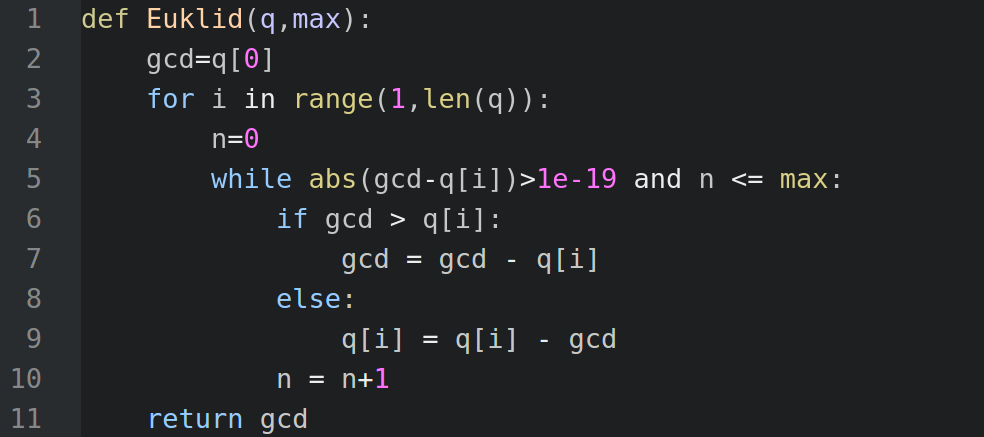
\includegraphics[height=6cm]{ressources/kot.png}
  \caption{Euklidischer Algorithmus für reelle Zahlen.}
  \label{kot}
\end{figure}

% \begin{appendix}
% \section{Messdaten}
% \centering
% \begin{figure}
% \includepdf[width=0.9\textwidth, pages={1}]{Bilder/Messdaten.pdf}
% \end{figure}
% \newpage
% \begin{figure}
% \includepdf[width=0.9\textwidth, pages={2}]{Bilder/Messdaten.pdf}
% \end{figure}
%
% \end{appendix}
